\thispagestyle{diendandayvahoctoannone}
\pagestyle{diendandayvahoctoan}
\everymath{\color{diendantoanhoc}}
\graphicspath{{../diendantoanhoc/pic/}}
\blfootnote{$^{1}$\color[named]{diendantoanhoc}Hà Nội.}
\begingroup
\AddToShipoutPicture*{\put(0,616){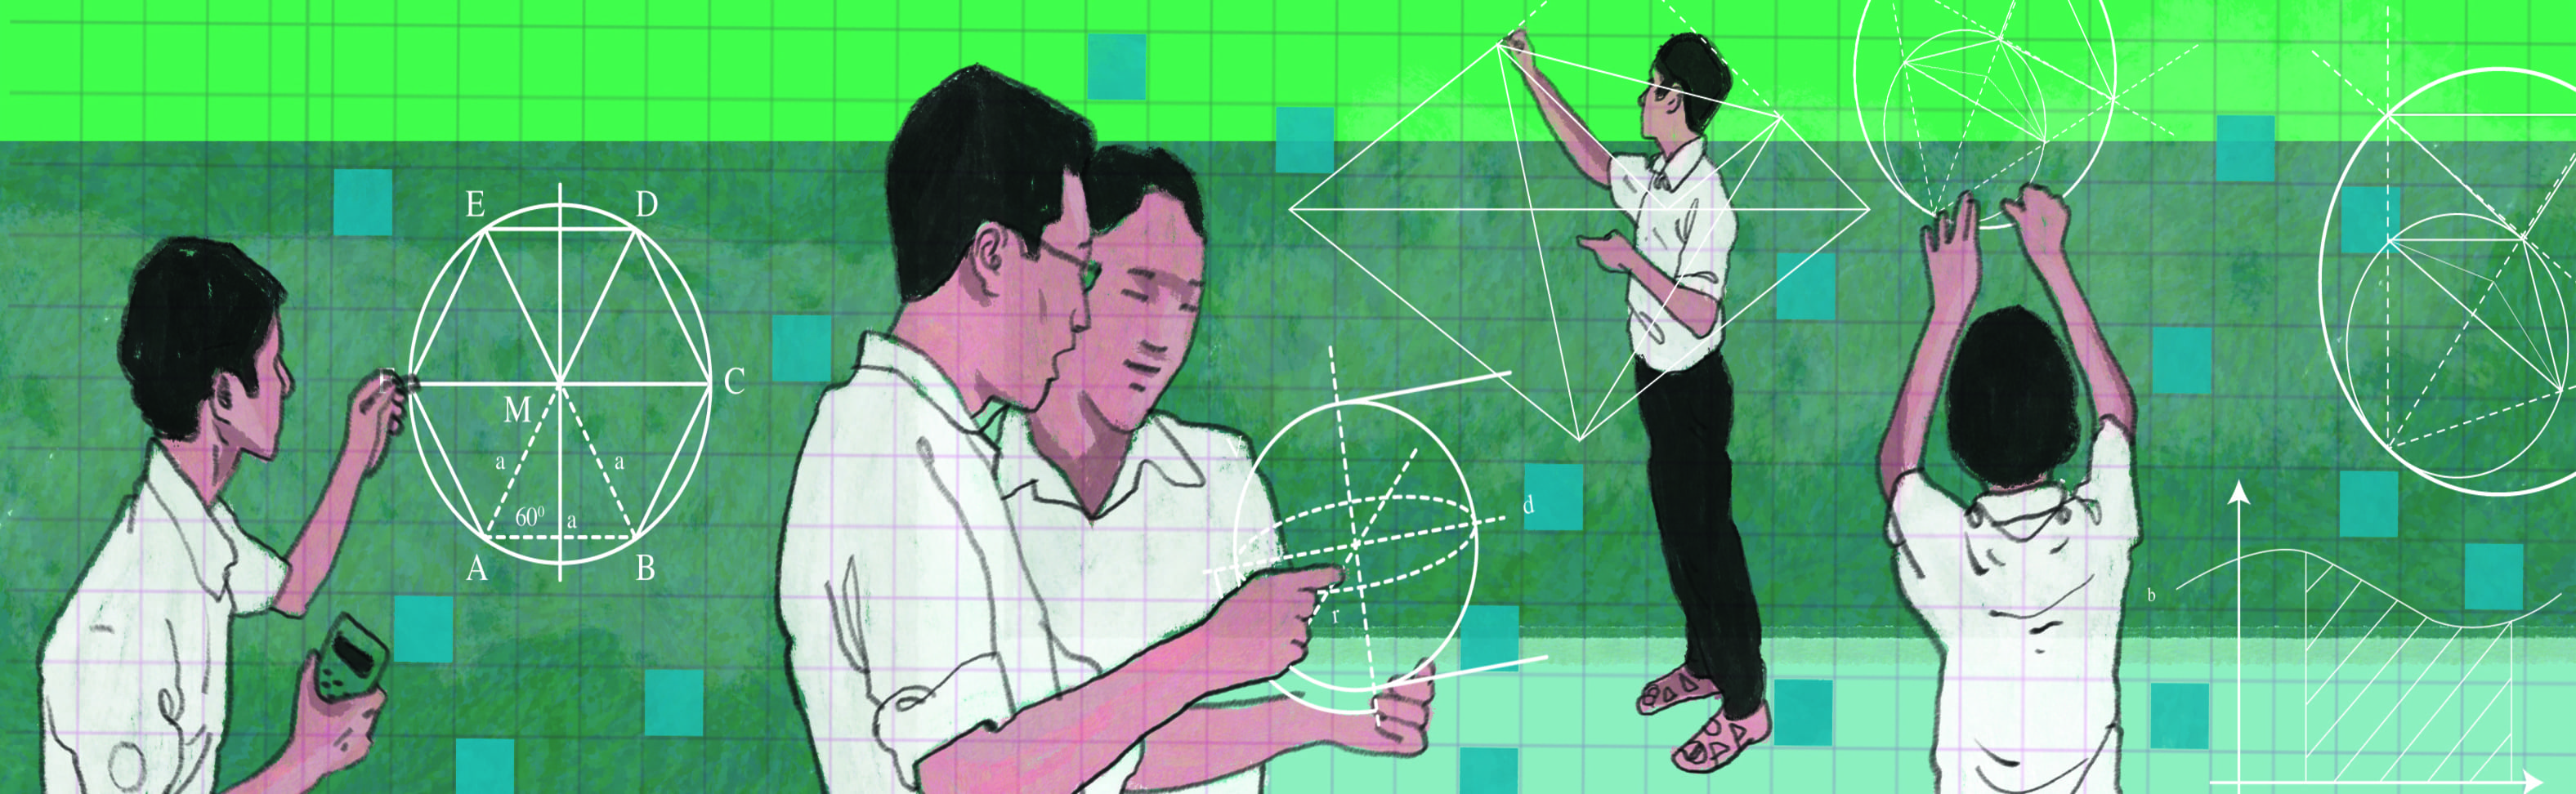
\includegraphics[width=19.3cm]{../bannerdiendan}}}
\AddToShipoutPicture*{\put(56,525){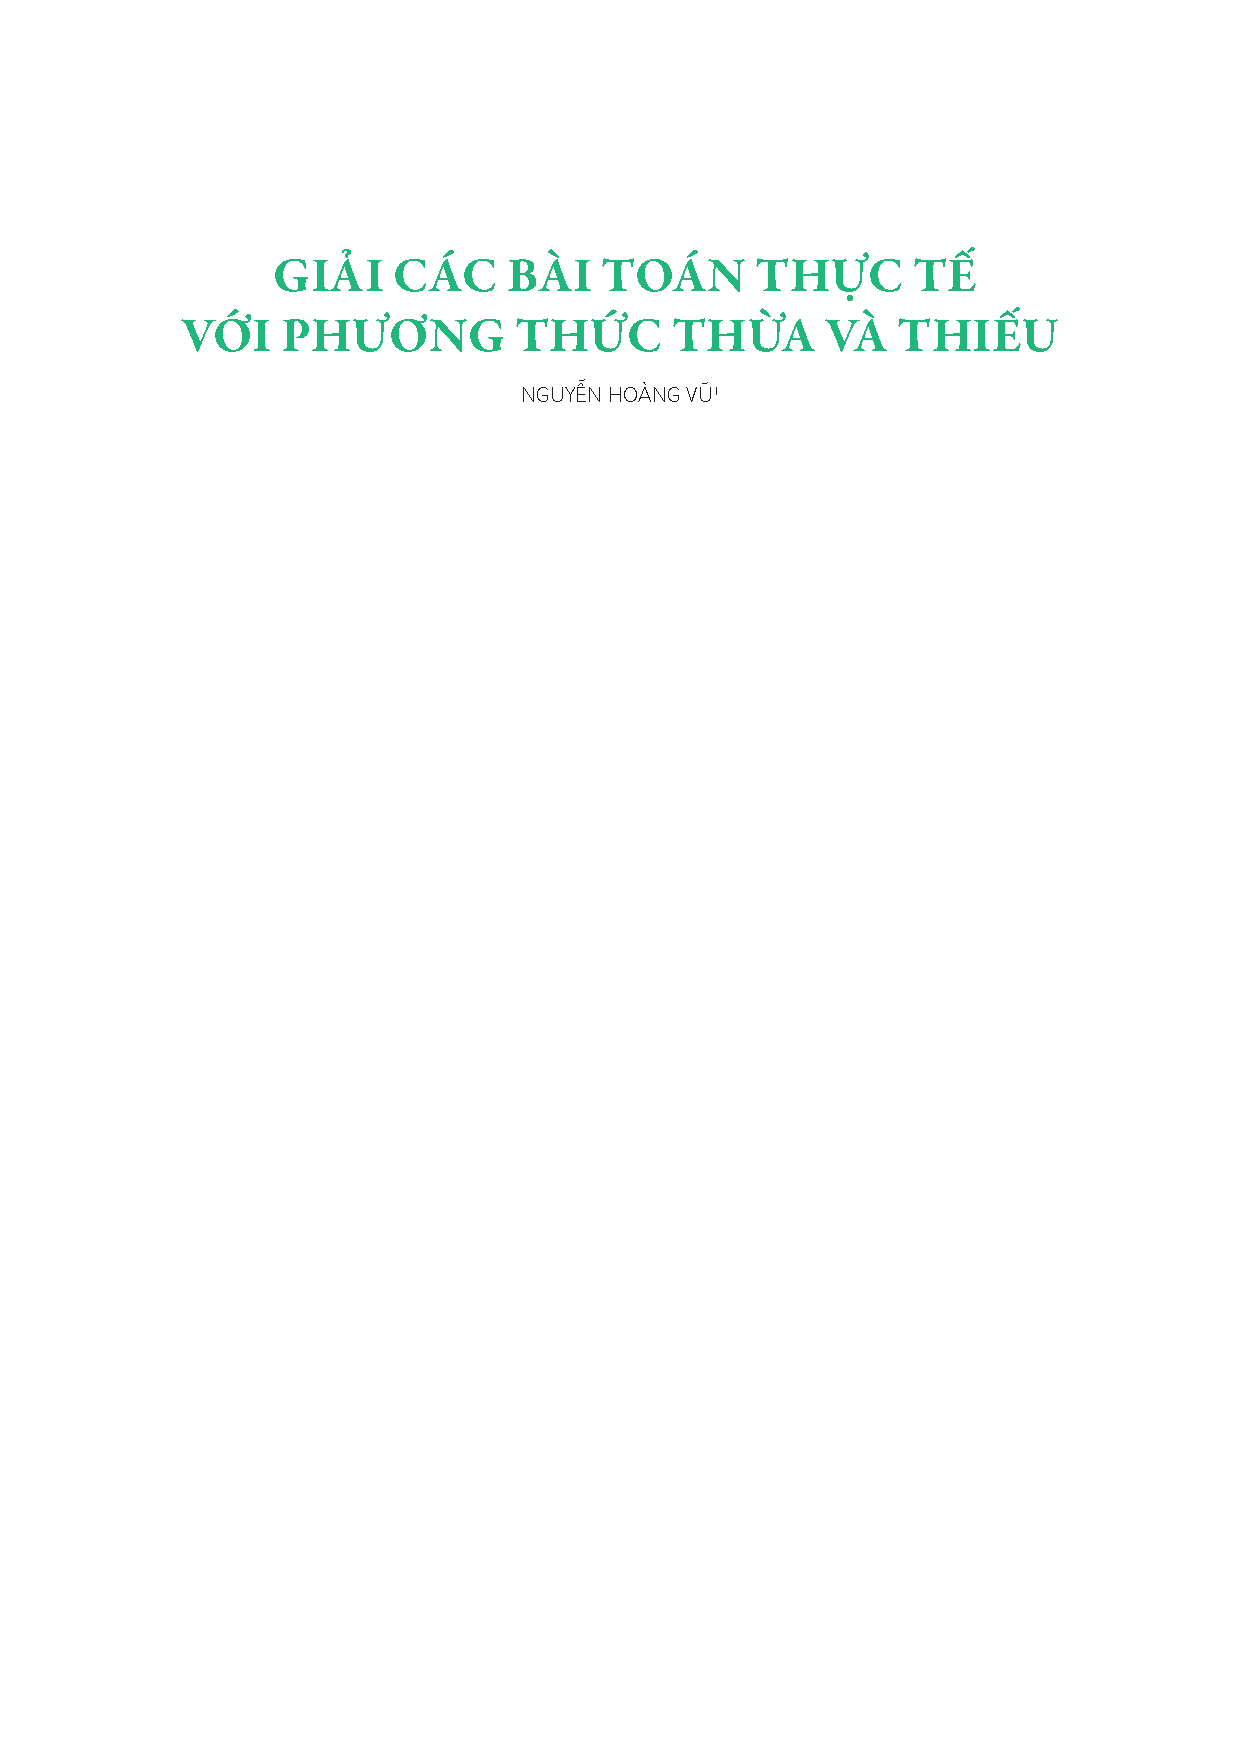
\includegraphics[scale=1]{../tieude.pdf}}}
\centering
\endgroup
\vspace*{185pt}

\begin{multicols}{2}
	Lưu Huy là một nhà toán học Trung Quốc nổi tiếng với cuốn sách \textit{Cửu chương toán thuật}. Trong đó, chương số $7$ mang tên ``\textit{Thừa và thiếu}" trình bày một phương pháp thú vị để giải các bài toán thực tế với nhiều ví dụ từ dễ đến khó. Bài viết này giới thiệu toàn bộ các bài tập trong chương này, trừ một số bài cuối là các bài toán tìm lời giải dạng gần đúng.
	\begin{figure}[H]
		\vspace*{-5pt}
		\centering
		\captionsetup{labelformat= empty, justification=centering}
		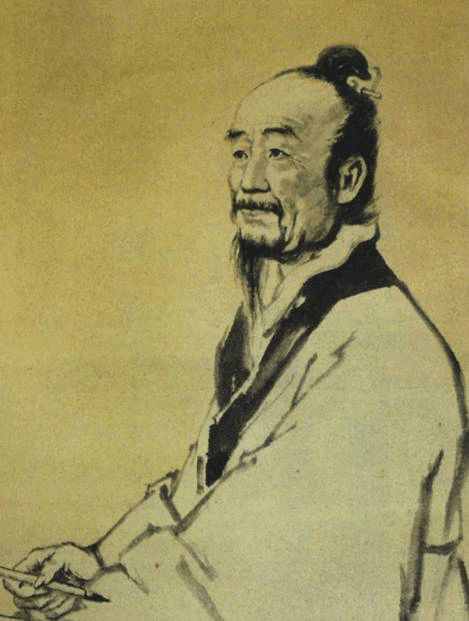
\includegraphics[width= 0.7\linewidth]{1}
		\caption{\small\textit{\color{diendantoanhoc}Lưu Huy ($220-280$.)}}
		\vspace*{-10pt}
	\end{figure}
	\textbf{\color{diendantoanhoc}Bài toán số $\pmb{1.}$} Một nhóm người góp tiền mua hàng. Nếu mỗi người bỏ ra $8$ đồng thì thừa $3$ đồng. Nếu mỗi người bỏ ra $7$ đồng thì thiếu $4$ đồng. Hỏi có bao nhiêu người và họ bỏ ra bao nhiêu tiền?
	\vskip 0.1cm
	\textit{Phương pháp:} Để giải bài toán này, trước hết ta cần thiết lập công thức cho bài toán tổng quát:
	\vskip 0.1cm
	Mỗi người bỏ ra $A$ đồng thì mua được toàn bộ lượng hàng và thừa ra $a$ đồng.
	\vskip 0.1cm
	Mỗi người bỏ ra $B$ đồng thì khi mua toàn bộ lượng hàng sẽ thiếu $b$ đồng.
	\vskip 0.1cm
	Phương pháp giải được tiến hành sao cho lượng tiền thừa và lượng tiền thiếu ở hai phát biểu bằng nhau. Ta lập luận như sau:
	\vskip 0.1cm
	Mỗi người bỏ ra $Ab$ đồng thì mua được $b$ lần lượng hàng và thừa ra $ab$ đồng.
	\vskip 0.1cm
	Mỗi người bỏ ra $aB$ đồng thì khi mua $a$ lần lượng hàng và thiếu $ab$ đồng.
	\vskip 0.1cm
	Khi cộng vào, lượng thừa và thiếu bằng nhau sẽ triệt tiêu hết, ta được:
	\vskip 0.1cm
	Mỗi người bỏ ra $Ab+aB$ đồng thì mua được vừa đủ $(a+b)$ lần lượng hàng.
	\vskip 0.1cm
	Do đó số tiền thực tế mỗi người bỏ ra khi mua hàng là: $\dfrac{Ab + aB}{a + b}$ $(1)$.
	\vskip 0.1cm
	Ta nhận thấy khi số tiền mỗi người bỏ ra thay đổi từ $A$ thành $B$ thì tổng số tiền tất cả mọi người bỏ ra sẽ thay đổi từ thừa $a$ thành thiếu $b$, tức là giảm đi một lượng $a+b$. Do đó, số người là:
	\begin{align*}
		m = \frac{a + b}{A-B}.
	\end{align*}
	Giá trị của lượng hàng sẽ bằng số tiền mỗi người bỏ ra nhân với số người, tức là:
	\begin{align*}
		\frac{Ab+ aB}{a + b} \cdot \dfrac{a+b}{A-B}= \frac{Ab+ aB}{A-B}.
	\end{align*}
	Lưu Huy cũng trình bày một cách giải thứ hai cho dạng toán này. Trong đó, số người được tính theo lập luận như trên còn giá trị hàng hóa được tính trực tiếp theo $n \cdot A - a$ hoặc $n \cdot B - b$.
	\vskip 0.1cm
	Cách giải thứ hai này ngắn hơn nhưng cách giải thứ nhất sẽ trợ giúp chúng ta giải được những bài toán phức tạp hơn tiếp theo.
	\vskip 0.1cm
	Việc cân bằng giữa đại lượng thừa và đại lượng thiếu là đặc trưng cơ bản của phương pháp này. Tên gọi đầy đủ của nó trong sách là ``doanh bất túc thuật" (doanh: tràn đầy, bất túc: không đủ, thuật: phương pháp).
	\vskip 0.1cm
	\textit{Đáp số}: Với dữ liệu của bài toán số $1$, ta có $A=8,a=3,B=7,b=4$. Thay vào công thức ta được số tiền mỗi người bỏ ra là $\frac{53}{7}$, số người là $7$, giá trị hàng hóa là $53$.
	\vskip 0.1cm
	\textbf{\color{diendantoanhoc}Bài toán số $\pmb{2.}$} Cùng mua gà, mỗi người trả $9$ thì thừa $11$, mỗi người trả $6$ thì thiếu $16$. Hỏi có bao nhiêu người và gà giá bao nhiêu.
	\vskip 0.1cm
	\textit{Đáp số}: Làm tương tự bài số $1$, ta được đáp án là $9$ người và giá trị số gà là $70$.
	\vskip 0.1cm
	Bài số $3$ và bài số $4$ tương tự bài số $1$ và bài số $2$ nhưng có sự xuất hiện của phân số. Bạn đọc có thể tự giải. Lưu Huy còn đưa ra phương pháp kết hợp việc quy đồng mẫu số vào trong quá trình giải, nhưng cách làm này phức tạp hơn và không quá cần thiết do học sinh đã quen thuộc với tính toán phân số nên sẽ không trình bày ở đây.
	\vskip 0.1cm
	\textbf{\color{diendantoanhoc}Bài toán số $\pmb{3.}$} Mỗi người bỏ ra $\dfrac{1}{2}$ đồng thì thừa $4$. Mỗi người bỏ ra $\dfrac{1}{3}$ đồng thì thiếu $3$. Hỏi có bao nhiêu người và giá mua là bao nhiêu?
	\vskip 0.1cm
	\textbf{\color{diendantoanhoc}Bài toán số $\pmb{4.}$} Hôm nay người ta cùng mua bò. Nếu cứ mỗi $7$ hộ trả chung $190$ thì thiếu $330$. Nếu mỗi $9$ hộ trả chung $270$ thì thừa $30$. Hỏi có bao nhiêu hộ và giá bò là bao nhiêu?
	\vskip 0.1cm
	\textbf{\color{diendantoanhoc}Bài toán số $\pmb{5.}$} Hôm nay người ta cùng mua vàng. Mỗi người bỏ ra $400$ thì thừa $3400$. Mỗi người bỏ $300$ thì thừa $100$. Hỏi có bao nhiêu người và giá vàng là bao nhiêu?
	\vskip 0.1cm
	\textit{Phương pháp:}
	\vskip 0.1cm 
	Bắt đầu từ bài toán:
	\vskip 0.1cm
	Mỗi người bỏ ra $A$ đồng thì mua được toàn bộ lượng hàng và thừa ra $a$ đồng.
	\vskip 0.1cm
	Mỗi người bỏ ra $B$ đồng thì khi mua toàn bộ lượng hàng sẽ thừa $b$ đồng.
	\vskip 0.1cm
	Lập luận như sau:
	\vskip 0.1cm
	Mỗi người bỏ ra $Ab$ đồng thì mua được $b$ lần lượng hàng và thừa ra $ab$ đồng.
	\vskip 0.1cm
	Mỗi người bỏ ra $aB$ đồng thì khi mua $a$ lần lượng hàng và thừa $ab$ đồng.
	\vskip 0.1cm
	Thay vì cộng như trong bài số $1$ thì ta tiến hành trừ để hai lượng tiền thừa ra triệt tiêu nhau. Bạn đọc có thể tự hoàn thiện các công thức còn thiếu để cho ra đáp số.
	\vskip 0.1cm
	\textit{Đáp số:} $33$ người, giá vàng là $3800$.
	\vskip 0.1cm
	\textbf{\color{diendantoanhoc}Bài toán số $\pmb{6.}$} Hôm nay người ta cùng mua cừu. Nếu mỗi người trả $5$ thì thiếu $45$. Nếu mỗi người trả $7$ thì thiếu $3$. Hỏi có bao nhiêu người và giá cừu là bao nhiêu.
	\vskip 0.1cm
	\textit{Phương pháp:} Bài toán thiếu và thiếu này tương tự như bài toán thừa và thừa, bạn đọc có thể tự giải.
	\vskip 0.1cm
	\textbf{\color{diendantoanhoc}Bài toán số $\pmb{7.}$} Hôm nay người ta cùng mua chó. Nếu mỗi người trả $5$ thì thiếu $90$. Nếu mỗi người trả $50$ thì vừa đủ. Hỏi có bao nhiêu người và giá chó là bao nhiêu?
	\vskip 0.1cm
	\textit{Phương pháp:} Bài toán thiếu và đủ này có thể được giải tương tự bài toán thừa thiếu theo cách $2$ của bài số $1$, với $a=0$. Giá trị của số hàng có thể được tính trực tiếp theo công thức: $n\cdot B$.
	\vskip 0.1cm
	\textit{Đáp số:} Số người là $\dfrac{90}{50-5} = 2$. Giá chó là $2\cdot 50=100$.
	\vskip 0.1cm
	\textbf{\color{diendantoanhoc}Bài toán số $\pmb{8.}$} Hôm nay người ta cùng mua lợn. Nếu mỗi người trả $100$ thì thừa $100$. Nếu mỗi người trả $90$ thì vừa đủ. Hỏi có bao nhiêu người và giá lợn là bao nhiêu?
	\vskip 0.1cm
	\textit{Phương pháp:} Bài toán thừa và đủ cũng tương tự bài toán thiếu và đủ, khi giải ta cho $b=0$.
	\vskip 0.1cm
	\textit{Đáp số:} Số người là $\dfrac{100}{100-90}$. Giá lợn là $10\cdot90=900$.
	\vskip 0.1cm
	\textbf{\color{diendantoanhoc}Bài toán số $\pmb{9.}$} Giả sử có một lượng gạo đã xát trong một cái thùng $10$ đấu, không rõ là có bao nhiêu gạo. Đổ đầy thùng bằng kê chưa xát. Sau khi xát được $7$ đấu cả gạo lẫn kê đã xát. Biết mỗi đấu kê chưa xát sau khi xát được $6$ thăng (đơn vị đo thể tích: $1$ đấu = $10$ thăng). Hỏi ban đầu có bao nhiêu đấu gạo.
	\vskip 0.1cm
	\textit{Phương pháp:} Tuy phát biểu bài toán tương đối phức tạp, nhưng bài toán này có thể đưa về dạng thừa và thiếu, thừa và thừa hoặc thiếu và thiếu. Ta cần chọn hai giá trị bất kỳ cho số gạo ban đầu trong thùng để tiến hành thiết lập các giả định.
	\vskip 0.1cm
	Giả sử ban đầu có $1$ đấu gạo xát rồi trong thùng, vậy có $9$ đấu kê chưa xát. Sau khi xát được $1$ đấu gạo và $5$ đấu $4$ thăng kê. Tức là thiếu $6$ thăng so với thực tế.
	\vskip 0.1cm
	Giả sử ban đầu có $3$ đấu gạo xát rồi trong thùng, vậy có $7$ đấu kê chưa xát. Sau khi xát được $3$ đấu gạo và $4$ đấu $2$ thăng kê. Tức là thừa $2$ thăng so với thực tế.
	\vskip 0.1cm
	Quy tất cả về thăng, ta được bài toán thừa và thiếu với $A=30,a=2,B=10,b=6$.
	\vskip 0.1cm
	\textit{Đáp số:} Dùng công thức để tính số tiền mỗi người phải đóng trong bài số $1$, ta được số gạo ban đầu là: $\dfrac{30 \times 6 + 10\times 2}{2 +6}$ thăng tức $2$ đấu rưỡi.
	\vskip 0.1cm
	\textit{Nhận xét:} Trong bài toán số $1$, cách giải đầu tiên sử dụng công thức ($1$) có vẻ phức tạp hơn nhưng nó cho phép chúng ta tìm nhanh đáp án cho những bài toán phức tạp như bài toán số $9$ này. Tùy vào các giá trị giả định mà ta thu được một trong ba dạng bài toán thừa và thiếu, thừa và thừa hoặc thiếu và thiếu.
	\vskip 0.1cm
	\textit{Mở rộng:} Thuật toán của Lưu Huy trong bài toán này thực tế là phương pháp nội suy cho hàm số tuyến tính $y=ax+b$. Trong một số trường hợp, $a$ và $b$ không xuất hiện trong đầu bài nhưng ta có thể tính được $y$ khi biết $x$ theo một phương thức khác nào đó như trên. Ta có thể chọn hai giá trị bất kỳ $x_1,x_2$ của $x$, tính các giá trị $y_1,y_2$ tương ứng rồi dùng nội suy để xác định giá trị $x$ sao cho $y=0$ mà không cần tính trực tiếp $a$ và $b$. Ví dụ trong bài số $9$ trên, $x$ là số đấu gạo ban đầu còn $y$ là mức độ chênh lệch giữa số đấu lương thực còn lại sau khi xát của trường hợp giả định so với thực tế. Trong khi đó, phương pháp giả thiết tạm mà nhiều sách tham khảo cho học sinh giỏi giới thiệu để giải các bài toán như bài \textit{vừa gà vừa chó} dựa trên việc tìm một nghiệm thỏa mãn phương trình thứ nhất rồi thay đổi các biến nhưng vẫn giữ cho điều kiện này không đổi cho đến khi thỏa mãn điều kiện thứ hai. Với những trường hợp phức tạp hơn như bài số $9$, việc suy luận tìm ra áp dụng phương pháp giả thiết tạm là tương đối khó trong khi phương pháp thừa và thiếu có thể được áp dụng một cách trực tiếp. Việc chọn hai giá trị nào để sử dụng cho phương pháp thừa và thiếu là bất kỳ. Ta cũng có thể sử dụng cách chọn giá trị của phương pháp giả thiết tạm (tất cả $36$ con vật toàn là gà hoặc toàn là chó trong bài \textit{vừa gà vừa chó}): giả sử ban đầu $10$ đấu toàn là gạo, sau khi xát vẫn có $10$ đấu, thừa $3$ đấu so với thực tế; lại giả sử ban đầu tất cả là kê, sau khi xát được $6$ đấu, thiếu $1$ đấu so với thực tế. Khi đó: $A=100,a=30,B=0,b=10$. Cần chú ý rằng vào thời kỳ của Lưu Huy, toán học cổ Trung Quốc chưa có số $0$ đứng riêng biệt nên cách chọn như trên không xuất hiện trong chương $7$ của \textit{Cửu chương toán thuật}.
	\vskip 0.1cm
	\PIbox{
	Về mặt lịch sử, phương pháp sử dụng hai dự đoán không chính xác để từ đó tìm kết quả đúng cũng xuất hiện trong các tài liệu Arab thời Trung Cổ, với tên gọi \linebreak al--khatā'ayn (sai kép). Qua các công trình của Fibonacci, phương pháp này cũng xuất hiện ở châu Âu thế kỷ $13$ cũng với tên gọi này.}
	\vskip 0.1cm
	Bài toán chuyển động cũng có thể quy về dạng toán thừa và thiếu bằng cách giả định như bài số $9$. Những bài toán này có công thức giải trực tiếp thuận tiện hơn nhiều nhưng vẫn được trình bày ở đây làm tài liệu tham khảo cho bạn đọc (bài số $10$ và bài số $11$).
	\vskip 0.1cm
	\textbf{\color{diendantoanhoc}Bài toán số $\pmb{10.}$} Bức tường cao $9$ thước. Từ nóc tường, cây dưa mọc xuống dưới mỗi ngày $7$ tấc (đơn vị đo độ dài: $1$ thước = $10$ tấc). Từ chân tường, cây mướp mọc lên mỗi ngày $1$ thước. Hỏi sau bao nhiêu ngày chúng gặp nhau, và khi đó mỗi dây dài (cao) bao nhiêu?
	\vskip 0.1cm
	\textit{Phương pháp:} Ta cũng chọn hai giá trị thời gian bất kỳ để xét tính thừa thiếu.
	\vskip 0.1cm
	Giả sử thời gian hai cây đã mọc là $1$ ngày. Mỗi cây lần lượt mọc được $7$ tấc và $1$ thước, tổng cộng là $17$ tấc, thiếu $73$ tấc so với chiều cao của tường.
	\vskip 0.1cm
	Giả sử thời gian hai cây đã mọc là $10$ ngày. Mỗi cây lần lượt mọc được $70$ tấc và $10$ thước, tổng cộng là $170$ tấc, thừa $80$ tấc so với chiều cao của tường.
	\vskip 0.1cm
	Ta được bài toán thừa và thiếu với $A=1,a=73,B=10,b=80$.
	\vskip 0.1cm
	\textit{Đáp số:} Thời gian gặp nhau của hai cây là $\dfrac{1\times80 + 10\times73}{73 + 80} =5\dfrac{5}{17}$ ngày.
	\vskip 0.1cm
	\textbf{\color{diendantoanhoc}Bài toán số $\pmb{11.}$} Cây thứ nhất ngày đầu tiên mọc được $3$ thước. Cây thứ hai ngày đầu tiên mọc được một thước. Sau đó, mỗi ngày cây thứ nhất mọc một nửa so với ngày đầu còn cây thứ hai mọc gấp đôi ngày đầu. Hỏi sau bao lâu hai cây cao bằng nhau?
	\vskip 0.1cm
	\textit{Phương pháp:} Tương tự bài số $10$ nhưng ta đem so khoảng cách đã mọc của cây thứ hai với cây thứ nhất. Nếu nhỏ hơn thì là thiếu, nếu dài hơn thì là thừa. Bạn đọc có thể tự giải theo hướng này.
	\vskip 0.1cm
	\textit{Đáp số:} $2\dfrac{6}{13}$ ngày.
	\vskip 0.1cm
	\textbf{\color{diendantoanhoc}Bài số $\pmb{12.}$} Giả sử rằng một đấu rượu tốt có giá $50$ đồng còn một đấu rượu thường có giá $10$ đồng. Một người mua tổng cộng hai đấu rượu với giá $30$ đồng. Hỏi có bao nhiêu rượu tốt và rượu thường đã được mua.
	\vskip 0.1cm
	\textit{Phương pháp:} Bài này tương tự bài số $9$. Ta chọn hai giá trị cho lượng rượu tốt trong tổng số $2$ đấu rượu (ví dụ $1$ đấu và $2$ đấu) rồi so tổng số tiền với số tiền rượu trong thực tế ($30$ đồng). 
	\vskip 0.1cm
	\textit{Đáp số:} $2$ thăng rưỡi rượu tốt, $1$ đấu $7$ thăng rưỡi rượu thường.
	\vskip 0.1cm
	\textbf{\color{diendantoanhoc}Bài số $\pmb{13.}$} Giả sử rằng $5$ cái bình lớn và $1$ cái bình nhỏ chứa được $3$ hộc, $1$ cái bình lớn và $5$ cái bình nhỏ chứa được $2$ hộc. Hỏi mỗi bình lớn hoặc bình nhỏ chứa được bao nhiêu. (Chú thích: $1$ hộc = $10$ đấu).
	\vskip 0.1cm
	\textit{Phương pháp:} Lưu Huy đưa bài toán này về dạng thừa và thiếu như sau:
	\vskip 0.1cm
	Giả sử bình lớn chứa được $5$ đấu, bình nhỏ cũng sẽ là $5$ đấu (do $5$ lớn + $1$ nhỏ chứa được $3$ hộc). Khi đó $1$ nhỏ + $5$ lớn sẽ chứa được $3$ hộc, nhiều hơn $10$ đấu so với thực tế ($2$ hộc).
	\vskip 0.1cm
	Tương tự, nếu bình lớn chứa được $5$ đấu rưỡi (tức $5$ đấu $5$ thăng) thì $1$ nhỏ + $5$ lớn sẽ bị thiếu $2$ đấu so với thực tế ($2$ hộc).
	\vskip 0.1cm
	Bạn đọc có thể tự giải tiếp phần sau.
	\vskip 0.1cm
	\textit{Đáp số:} Bình lớn chứa được $\dfrac{13}{24}$ hộc. Bình nhỏ chứa được $\dfrac{7}{24}$ hộc.
	\vskip 0.1cm
	\textbf{\color{diendantoanhoc}Bài số $\pmb{14.}$} Giả sử có $3$ đấu sơn. Cứ $3$ thăng sơn đổi được $4$ thăng dầu, cứ $4$ thăng dầu trộn được với $5$ thăng sơn. Từ lượng sơn ban đầu, lấy ra một phần để đổi dầu đủ để trộn hết với lượng sơn còn lại. Hỏi phải lấy bao nhiêu sơn để đổi, thu được bao nhiêu dầu và trộn với bao nhiêu sơn?
	\vskip 0.1cm
	\textit{Phương pháp:} Tương tự bài số $9$, giả sử hai giá trị khác nhau cho lượng sơn đem đi đổi dầu rồi xét khi trộn thì sơn bị thừa hay thiếu.
	\vskip 0.1cm
	\textit{Đáp số:} Lấy $1$ đấu $\dfrac{11}{4}$ thăng sơn đi đổi. 
	\vskip 0.1cm
	Các bài số $15$, $16$, $17$, việc quy về dạng thừa và thiếu có thể tiến hành tương tự các bài trước, bạn đọc có thể tiến hành tự giải.
	\vskip 0.1cm
	\textbf{\color{diendantoanhoc}Bài số $\pmb{15.}$} Giả sử một khối ngọc hình lập phương có cạnh $1$ tấc thì nặng $7$ lượng, một khối đá hình lập phương có cạnh $1$ tấc thì nặng $6$ lượng. Giả sử ta có một khối đá lập phương cạnh $3$ tấc, bên trong có ngọc. Tổng khối lượng là $11$ cân ($1$ cân bằng $16$ lượng). Hỏi ngọc nặng bao nhiêu, đá nặng bao nhiêu?
	\vskip 0.1cm
	\textbf{\color{diendantoanhoc}Bài số $\pmb{16.}$} Một mẫu ruộng tốt giá $300$, $7$ mẫu ruộng xấu giá $500$. Người ta mua một khoảnh 100 mẫu với giá $1$ vạn đồng. Hỏi có bao nhiêu ruộng tốt và bao nhiêu ruộng xấu?
	\vskip 0.1cm
	\textbf{\color{diendantoanhoc}Bài số $\pmb{17.}$} Giả sử $9$ thanh vàng nặng bằng $11$ thanh bạc. Sau khi đổi $1$ thanh vàng thành $1$ thanh bạc, bạc nặng hơn vàng là $13$ lượng. Hỏi ban đầu mỗi loại nặng bao nhiêu?
	\vskip 0.1cm
	Các bài toán thừa và thiếu cũng xuất hiện nhiều trong các tài liệu Hán Nôm cổ của Việt Nam. Nhiều bài toán từ các nguồn này đã được PGS. TS. Tạ Duy Phượng giới thiệu trong các số $188+189$, $192+193$, và $209+210$ của tạp chí Toán Tuổi thơ $2$. Bạn đọc có thể tìm những số này để tham khảo thêm. Các bài toán trong bài viết cũng đã được tác giả giảng dạy cho lớp K$3$ của câu lạc bộ Toán học UMC do Pi và Viện Toán học phối hợp tổ chức. Hiện nay, \textit{Cửu chương toán thuật} đã có các bản dịch ra nhiều ngôn ngữ nhưng chưa có bản tiếng Việt. Những nội dung khác có giá trị cho việc dạy và học toán từ cuốn sách này sẽ tiếp tục được Pi giới thiệu với độc giả khi có điều kiện.
	\vskip 0.1cm
	\textbf{\color{diendantoanhoc}Tài liệu tham khảo}
	\vskip 0.1cm
	[$1$] Boman, E. C. ($2009$). False Position, Double False Position and Cramer's Rule. \textit{The College Mathematics Journal}, $40(4)$, $279-283$. \url{https://doi.org/10.4169/193113409x458732}
	\vskip 0.1cm
	[$2$] Schwartz, R. K. ($2004$). \textit{Issues in the Origin and Development of Hisāb al--Khatā'ayn (Calculation by Double False Position)}. Presented at the Eighth Maghrebian Colloquium on the History of Arab Mathematics (COMHISMA$8$), Radès, Tunisia.
\end{multicols}
\vspace*{-10pt}
{\color{diendantoanhoc}\rule{1\linewidth}{1pt}}
\vskip 0.2cm
\centerline{\Large{\textbf{\color{diendantoanhoc}LỜI GIẢI, ĐÁP ÁN}}}
\vskip 0.1cm
\begin{multicols}{2}
	\textbf{\color{diendantoanhoc}Đố vui}
	\vskip 0.1cm
	Buratino có thể chia $15$ đồng xu của mình thành $3$ nhóm với số lượng xu tương ứng là $7, 4,4$;  $5, 5, 5$; $3, 6, 6$ hoặc $1, 7, 7$.
	\vskip 0.1cm
	Ở lần cân thứ nhất, Buratino đặt $2$ nhóm xu có số lượng bằng nhau lên $2$ đĩa cân. Xét trường hợp cân thăng bằng. Khi này tất cả các đồng xu trong $2$ nhóm đó là các đồng xu thật và đồng xu giả nằm ở nhóm còn lại. Sau đó, ở lần cân thứ hai, Buratino đặt nhóm đồng xu chứa đồng xu giả lại lên $1$ chiếc đĩa và đặt lên chiếc đĩa còn lại một số đồng xu (lấy từ $2$ nhóm chỉ đã cân) bằng với số đồng xu của nhóm chứa đồng xu giả. Như vậy, nếu nhóm chứa đồng xu giả nặng hơn thì đồng xu giả là của Basile còn nếu nhẹ hơn thì là của Alice. Xét trường hợp cân không thăng bằng ở lần cân đầu tiên. Khi này tất cả các đồng xu ở nhóm còn lại là thật. Ở lần cân thứ $2$, Buratino bỏ các đồng xu ở bên nhẹ hơn ra khỏi đĩa và chia các đồng xu ở bên nặng hơn
	\vskip 0.1cm
	\hfill \textit{(Xem tiếp trang $39$)}
\end{multicols}